\documentclass[12pt]{article}
\usepackage[utf8]{inputenc}
\usepackage{longtable}
\usepackage{multirow}
\usepackage{graphicx}
\graphicspath{ {./author/} }

\renewcommand{\baselinestretch}{1.5}

\title{Alonzo Church(1903-1995)}
\author{Luis Diego Jiménez Delgado}
\date{Agosto 12 del 2019}

\begin{document}

\maketitle

\begin{center}
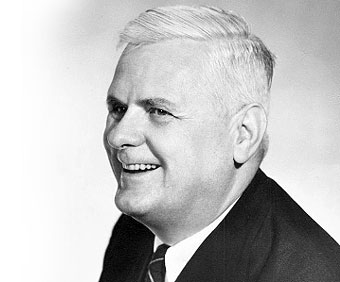
\includegraphics{ch}
\end{center}
Matemático y lógico estadounidense creador de la base de la computación teórica. Nacido en la ciudad de Washington, se diplomó en 1924 y obtuvo su doctorado en 1927 en la Universidad de Princeton, donde ejerció como profesor entre 1929 y 1967.
Su obra más conocida es el desarrollo del cálculo lambda, y su trabajo de 1936 que muestra la existencia de problemas indecidibles. Este trabajo precedió el famoso trabajo de su alumno Alan Turing sobre el problema de parada que también demostró la existencia de problemas irresolubles por dispositivos mecánicos. Luego de revisar la tesis doctoral de Turing, demostraron que el cálculo lambda y la máquina de Turing utilizada para expresar el problema de parada tenían igual poder de expresión; posteriormente demostraron que una variedad de procesos mecánicos alternos para realizar cálculos tenían poder de cómputo equivalente. Como resultado se postuló la Tesis de Church-Turing.
Entre los más conocidos estudiantes de doctorado de Church están Stephen Kleene, J. Barkley Rosser, Leon Henkin, John George Kemeny, Michael O. Rabin, Dana Scott, Simon Kochen y Raymond Smullyan.
Church publicó entre 1924 y 1995 trabajos sobre Lógica, filosofía, matemáticas y computación. En su trabajo de 1936 An unsolvable problem of elementary number theory Church formuló por primera vez lo que ahora se conoce como la tesis de Church que es la identificación del concepto vago de calculabilidad efectiva con la noción precisa de función recursiva. Su artículo A note on the entscheidungsproblem presentó lo que ahora se conoce como el teorema de Church: La indecidibilidad de la validez de la lógica de primer orden. En 1941 publicó su monografía The calculi of lambda-conversión. Este trabajo tiene gran influencia en el área de computación teórica.
El cálculo lambda influenció el diseño del lenguaje Lisp así como los lenguajes de programación funcional.
\end{document}